% Options for packages loaded elsewhere
\PassOptionsToPackage{unicode}{hyperref}
\PassOptionsToPackage{hyphens}{url}
\documentclass[
  ignorenonframetext,
]{beamer}
\newif\ifbibliography
\usepackage{pgfpages}
\setbeamertemplate{caption}[numbered]
\setbeamertemplate{caption label separator}{: }
\setbeamercolor{caption name}{fg=normal text.fg}
\beamertemplatenavigationsymbolsempty
% remove section numbering
\setbeamertemplate{part page}{
  \centering
  \begin{beamercolorbox}[sep=16pt,center]{part title}
    \usebeamerfont{part title}\insertpart\par
  \end{beamercolorbox}
}
\setbeamertemplate{section page}{
  \centering
  \begin{beamercolorbox}[sep=12pt,center]{section title}
    \usebeamerfont{section title}\insertsection\par
  \end{beamercolorbox}
}
\setbeamertemplate{subsection page}{
  \centering
  \begin{beamercolorbox}[sep=8pt,center]{subsection title}
    \usebeamerfont{subsection title}\insertsubsection\par
  \end{beamercolorbox}
}
% Prevent slide breaks in the middle of a paragraph
\widowpenalties 1 10000
\raggedbottom
\AtBeginPart{
  \frame{\partpage}
}
\AtBeginSection{
  \ifbibliography
  \else
    \frame{\sectionpage}
  \fi
}
\AtBeginSubsection{
  \frame{\subsectionpage}
}
\usepackage{iftex}
\ifPDFTeX
  \usepackage[T1]{fontenc}
  \usepackage[utf8]{inputenc}
  \usepackage{textcomp} % provide euro and other symbols
\else % if luatex or xetex
  \usepackage{unicode-math} % this also loads fontspec
  \defaultfontfeatures{Scale=MatchLowercase}
  \defaultfontfeatures[\rmfamily]{Ligatures=TeX,Scale=1}
\fi
\usepackage{lmodern}
\ifPDFTeX\else
  % xetex/luatex font selection
\fi
% Use upquote if available, for straight quotes in verbatim environments
\IfFileExists{upquote.sty}{\usepackage{upquote}}{}
\IfFileExists{microtype.sty}{% use microtype if available
  \usepackage[]{microtype}
  \UseMicrotypeSet[protrusion]{basicmath} % disable protrusion for tt fonts
}{}
\makeatletter
\@ifundefined{KOMAClassName}{% if non-KOMA class
  \IfFileExists{parskip.sty}{%
    \usepackage{parskip}
  }{% else
    \setlength{\parindent}{0pt}
    \setlength{\parskip}{6pt plus 2pt minus 1pt}}
}{% if KOMA class
  \KOMAoptions{parskip=half}}
\makeatother
\setlength{\emergencystretch}{3em} % prevent overfull lines
\providecommand{\tightlist}{%
  \setlength{\itemsep}{0pt}\setlength{\parskip}{0pt}}
\usepackage{bookmark}
\IfFileExists{xurl.sty}{\usepackage{xurl}}{} % add URL line breaks if available
\urlstyle{same}
\hypersetup{
  hidelinks,
  pdfcreator={LaTeX via pandoc}}

\author{\texorpdfstring{}{}}
\date{}

\begin{document}

\begin{frame}[fragile]{Supplement: Layout and pipeline}
\protect\phantomsection\label{supplement-layout-and-pipeline}
\begin{figure}[!ht]
\centering
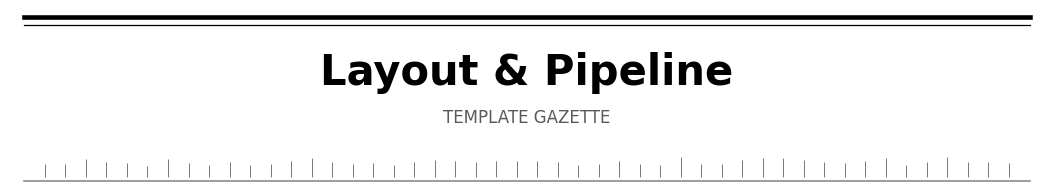
\includegraphics[width=\linewidth]{../figures/section_banner_S01_layout_and_pipeline.png}
\caption{Supplement banner marking the layout-and-pipeline desk; monochrome PNG from \texttt{generate\_section\_banners.py}.}
\label{fig:banner_S01_layout_and_pipeline}
\end{figure}
\begin{figure}[!ht]
\centering
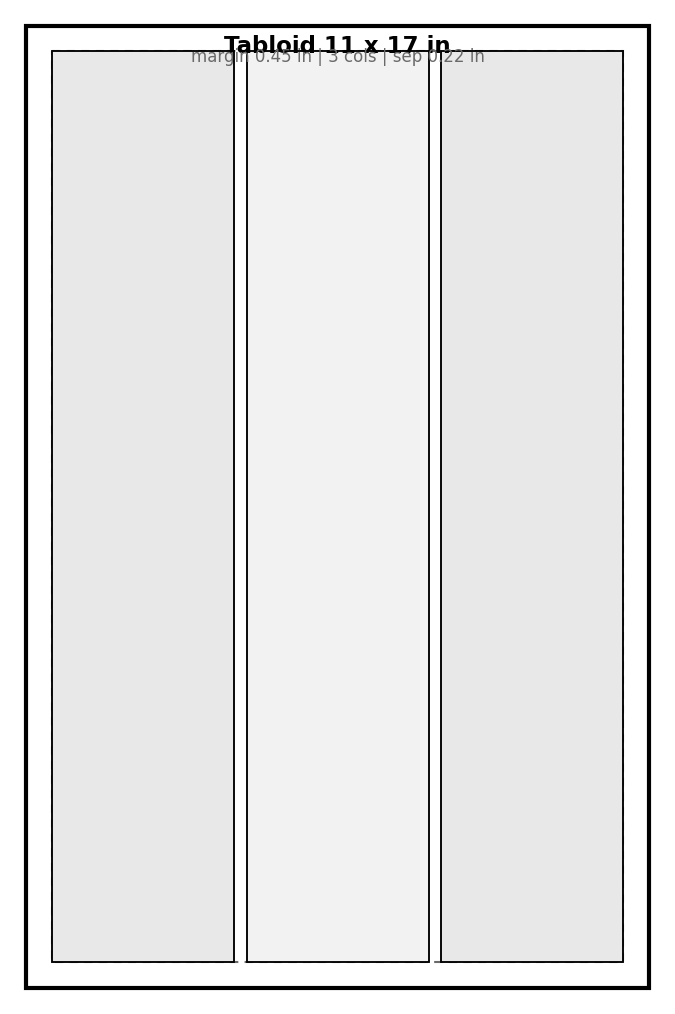
\includegraphics[width=0.92\linewidth]{../figures/layout_schematic.png}
\caption{Not to scale schematic from NewspaperLayout: tabloid sheet, dashed box is text area inside margins, shaded regions are three body columns with gutters. Values align with preamble geometry and layout\_spec.py.}
\label{fig:layout_schematic}
\end{figure}
\begin{multicols}{3}

\textbf{How this PDF is built.} Sixteen markdown slices under
\texttt{projects/traditional\_newspaper/manuscript/} are discovered by
\texttt{infrastructure.rendering.manuscript\_discovery.discover\_manuscript\_files},
combined in stem order, and separated by
\texttt{\textbackslash{}newpage} inside
\texttt{infrastructure.rendering.pdf\_renderer.PDFRenderer} before
Pandoc emits LaTeX. Tabloid paper (11 in × 17 in) and
\texttt{\textbackslash{}usepackage\{multicol\}} come from
\texttt{manuscript/preamble.md}; column separation matches
\texttt{src/newspaper/layout\_spec.py}
(\texttt{LAYOUT.column\_sep\_in}).
Figure\textasciitilde{}\ref{fig:layout_schematic} (above this column
block) summarizes the same numbers as a grid diagram.

The masthead PNG is produced by \texttt{scripts/generate\_masthead.py}
calling \texttt{newspaper.masthead.render\_masthead\_png} during Stage
02 analysis. Optional environment variables \texttt{NEWSPAPER\_TITLE}
and \texttt{NEWSPAPER\_TAGLINE} override banner text without editing
Python. In the combined PDF it is captioned as
Figure\textasciitilde{}\ref{fig:masthead}. A companion schematic ships
from \texttt{scripts/generate\_layout\_schematic.py} via
\texttt{render\_layout\_schematic\_png}, giving a second captioned
figure for float and caption testing.

\textbf{Stage ordering (core pipeline).} \texttt{execute\_pipeline.py}
and \texttt{./run.sh\ -\/-core-only} run, among others: environment
setup, tests, analysis scripts (including both figure generators when
present), PDF rendering, validation, and output copy. Analysis writes
into \texttt{projects/traditional\_newspaper/output/}; copy stages
mirror selected artifacts into \texttt{output/traditional\_newspaper/}
for distribution. Exact stage labels appear in console logs with
progress markers.

\textbf{Manuscript combination.} Each slice file is read as UTF-8 text.
Preamble metadata from \texttt{preamble.md} injects geometry and
packages. Title page fields derive from \texttt{config.yaml}
(\texttt{paper.title}, authors, version, date). Bibliography entries
live in \texttt{references.bib};
\texttt{\textbackslash{}cite\{template2026gazette\}} appears on the
front page and here to exercise BibTeX wiring.

\textbf{Word counts.} \texttt{scripts/report\_manuscript\_stats.py}
walks \texttt{all\_tracked\_manuscript\_basenames()} and emits
\texttt{output/data/manuscript\_stats.json} with per-file words, lines,
and bytes. CI or humans can diff that JSON across branches to catch
accidental truncation. It is a thin orchestrator: no analytics logic
beyond counting.

\textbf{Why tabloid.} The 11×17 inch choice stresses wide measure and
long vertical flow compared to letter paper. Three columns mimic
newspaper grids while remaining simple \texttt{multicol}
environments---no custom column balancers. If you shrink paper, update
\texttt{NewspaperLayout} constants, regenerate
\texttt{layout\_schematic.png}, and rerun tests that assert geometry
text in captions still matches code.

\textbf{Floats versus multicol.} Standard \texttt{figure} floats are not
supported inside \texttt{multicols}; the layout schematic therefore sits
before \texttt{\textbackslash{}begin\{multicols\}\{3\}} in this slice,
matching the front page pattern (masthead float, then three-column
body). Use \texttt{\textbackslash{}includegraphics} without a float if
you ever need art mid-column.

\textbf{Slides and web.} The same stems feed Beamer slides and HTML web
output via infrastructure renderers. Figure captions pass through Lua
filters for HTML; keep \texttt{\textbackslash{}caption\{\}} text free of
unmatched braces so extraction regexes succeed.

\textbf{Checkpointing and resume.} Root pipeline scripts support
checkpoints so long builds can restart after transient failures.
Newspaper builds are shorter than some monographs, but CI timeouts still
happen---resume flags save compute. Read
\texttt{docs/operational/config/checkpoint-resume.md} for semantics;
behavior is uniform across projects.

\textbf{Multi-project runs.} \texttt{./run.sh\ -\/-all-projects}
executes many exemplars sequentially. Infrastructure tests may run once
up front. When debugging \texttt{traditional\_newspaper} alone, pass
\texttt{-\/-project\ traditional\_newspaper} to avoid unrelated failures
blocking iteration.

\textbf{Environment variables.} Beyond masthead overrides,
\texttt{LOG\_LEVEL} tunes verbosity, \texttt{MPLBACKEND=Agg} ensures
headless matplotlib, and \texttt{PROJECT\_DIR} helps scripts resolve
paths when invoked from unexpected working directories. Document any new
vars in \texttt{scripts/AGENTS.md}.

\textbf{BibTeX keys.} \texttt{template2026gazette} in
\texttt{references.bib} exists to exercise citation machinery. Replace
with your publication entry when forking; keep keys ASCII and stable so
diffs stay readable.

\textbf{Figure path normalization.}
\texttt{\_pdf\_tex\_transforms.fix\_figure\_paths} rewrites
\texttt{../output/figures/} to \texttt{../figures/} relative to the
compile directory inside \texttt{output/.../pdf/}. If you add figures,
place PNGs under
\texttt{projects/traditional\_newspaper/output/figures/} before copy, or
under final \texttt{output/traditional\_newspaper/figures/} after
pipeline---know which stage consumes which path.

\textbf{Extending slice count.} If you truly need seventeen core folios,
you must edit \texttt{PAGE\_SLICES}, rename files, and update every test
asserting \texttt{16}. Prefer supplemental \texttt{S*} files for extra
prose---it avoids renumbering tourism.

\textbf{Teaching use.} Instructors can assign students to modify one
slice, regenerate PDFs, and explain diff in log output. The constrained
structure makes grading objective: does inventory pass? do captions
resolve? do tests stay green?

\textbf{Handover checklist (extended).} Before merging a layout change,
capture: (1) \texttt{git\ diff} on \texttt{preamble.md} and
\texttt{layout\_spec.py}, (2) regenerated \texttt{layout\_schematic.png}
if constants moved, (3) \texttt{manuscript\_stats.json} after
\texttt{report\_manuscript\_stats.py}, (4) PDF validator output excerpt
showing zero \texttt{??} references, (5) a one-line note in the PR
describing float behavior on the front page. Reviewers use the checklist
to avoid approving partial state where code and figures disagree.

This supplemental folio appears \textbf{after} the sixteen edition pages
and \textbf{before} the glossary slice, per the template's ordering:
main numeric sections, then \texttt{S*}, then \texttt{98\_*}, then
\texttt{99\_*} if present.

\noindent For citation metadata see \cite{template2026gazette}.
\par\smallskip

\end{multicols}
\end{frame}

\end{document}
